\documentclass[a4paper,12pt]{book}

\usepackage{url}
\usepackage[brazil]{babel}
\usepackage[pdftex]{graphicx}
\usepackage[pdftex]{hyperref}

\title{Xadrez em Realidade Aumentada - Manual}
\author{
		Douglas Bettioli Barreto (NUSP 6920223)
		\and Giancarlo Rigo (NUSP 6910034)
		\and Rafael Reggiani Manzo (NUSP 6797150)
	   }

\begin{document}

\maketitle

\part{Manual do usu\'ario}
\label{part:manualdousuario}
	\chapter{Introdu\c c\~ao}
	Para rodar o programa, o usuário far\'a uso do makefile, arquivo que ser\'a
	utilizado pelo programa make, que ir\'a compilar o programa. Para rodar o make,
	basta acessar o diret\'orio aonde está o arquivo “makefile” pelo terminal e
	digitar make. \'E importante ressaltar que para a identifica\c c\~ao das tags,
	a c\^amera deve ser posicionada com direção vertical \` superf\'cie das tags, preferencialmente em locais com boa iluminação e em superf\'icies planas.

\part{Manual do Desenvolvedor}
\label{part:manualdodesenvolvedor}
	\chapter{Diagrama de classes}
	\label{ch:diagramadeclasses}
	\begin{figure}[h]
	\centering
	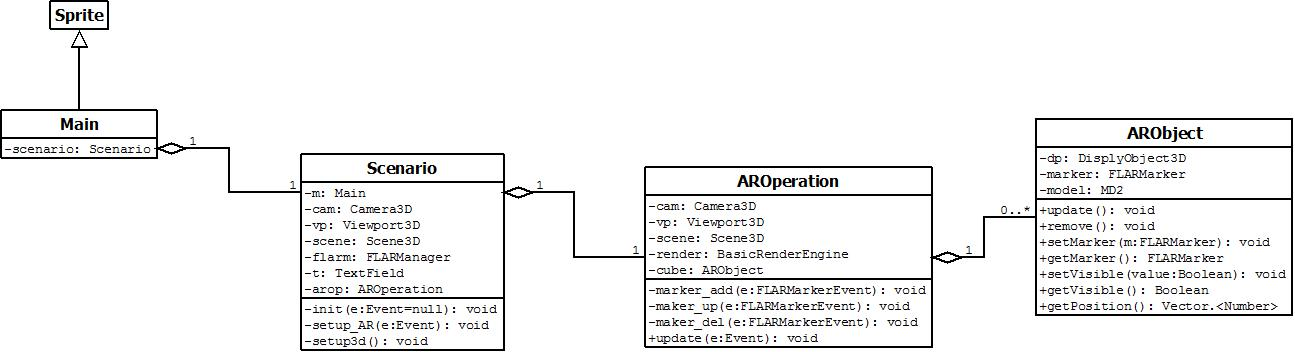
\includegraphics[width=1.2\textwidth]{diagramadeclasses}
	\end{figure}
	\footnote{Ver observacoes sobre a clase AROperation em
			  \ref{subsec:ecclassearoperation}
			 }
			 
	\chapter{Estrutura do c\'odigo}
	\label{ch:estruturadocodigo}
	
	\section{Compila\c c\~ao}
	\label{sec:eccompilacao}
	Este software foi desenvolvido e testado em Linux Ubuntu 10.04 (32 bits). Mas,
	teoricamente, deve funcionar em qualquer maquina que atenda aos requisitos
	(\ref{subsec:ecrequisitos})
	
	\subsection{Requisitos}
	\label{subsec:ecrequisitos}
	\begin{itemize}
		\item{Adobe Flex Compiler (mxmlc) Version 4.1.0 build 16076}
	\end{itemize}
	
	\subsection{Makefile}
	Encontrado dentro da pasta src. Dentro dele substitua o caminho para o mxmlc do
	seu Flex SDK.
	Existem duas op\c c\~oes de debug:
	\begin{itemize}
	  \item{Compilar a vers\~ao de produ\c c~ao: ``make''}
	  \item{Compilar a vers\~ao de debug: ``make debug''}
	\end{itemize}
	
	\section{Pacote principal}
		\label{sec:pcpacoteaugmentedreality}
		
		No momento, este pacote possui as classes Main e Scenario. Mas, com o
		desenvolvimento do projeto, devem ser criadas novas classes.
		
		\subsection{Classe Main}
		\label{subsec:ecclassemain}
		Esta classe simplesmente instancia um objeto da classe
		Scenario (\ref{subsec:ecclassescenario}).
		
		\subsection{Classe Scenario}
		\label{subsec:ecclassescenario}
		Esta classe recebe a inst\^ancia da classe Main na qual vai adicionar v\'arios
		``eventlistener'' e adicionar elementos como c\^amera, textos e boto\~oes. Seu
		objetivo \'e retirar do Main o c\'odigo que manipula a parte visual da
		aplica\c c\~ao.
		Trabalhando com a parte visual, esta classe n\~ao poderia deixar de utilizar
		classes do pacote de realidade aumentada (\ref{sec:pcpacoteaugmentedreality}).
		Vale ressaltar que os nomes de m\'etodos desta classe est\~ao muito ruins, mas
		a refatora\c c\~ao disto j\'a foi planejada para a pr\'oxima fase.
		\footnote{Link para a story da refatora\c c\~ao no pivotal:	\url{http://www.pivotaltracker.com/story/show/5588098}}
		
	\section{Pacote AugmentedReality}
		\label{sec:pcpacoteaugmentedreality}
		
		No momento, este pacote possui as classes ARObject e AROperation. Mas, com o
		desenvolvimento do projeto, devem ser criadas novas classes.
		
		\subsection{Classe AROperation}
		\label{subsec:ecclassearoperation}
		Esta classe concentra as opera\c c\~oes do FLARManager, como criar novos
		objetos de realidade aumentada atrav\'es da classe ARObject
		(\ref{subsec:ecclassearobject}) e atualizar os markers.
		No momento, esta classe deve ter um atributo para cada modelo 3D que deve ser
		mostrado. Mas, ja esta planejada a refatora\c c\~ao desta classe para que um
		array din\^amico substitua esta necessidade de v\'arios atributos
		(\footnote{Link para a story da refatora\c c\~ao no	pivotal: \url{http://www.pivotaltracker.com/story/show/5588098}}).
		
		
		\subsection{Classe ARObject}
		\label{subsec:ecclassearobject}
		Respons\'avel por carregar o modelo 3D do objeto, guardar seu marker e seu
		display. Nesta classe sao encontrados m\'etodos de get e set, por enquanto
		p\'ublicos\footnote{Dependendo do desenvolvimento do projeto estes m\'etodos
		podem se tornar protected e ser criada uma classe de interface para o pacote},
		para quase todos seus atributos. Ela \'e a classe mais b\'asica que temos hoje
		no software, sendo muito utilizada pela classe AROperation (\ref{subsec:ecclassearoperation}).
		
	\chapter{Prova de conceito}
	\label{ch:provadeconceito}
		\section{Introdu\c c\~ao}
		\label{sec:pcintroducao}
		A prova de conceito consistiu em abordar os pontos chave do projeto no que se
		refere a realidade aumentada. Nela, foram tratados temas como o reconhecimento
		de multiplos marcadores e a capacidade de obter as coordenadas do marcador no
		espa\c co. \footnote{A prova de conceito \'e o branch ``12 tags ao mesmo
		tempo" do reposit\'orio}
		
		\section{Marcadores}
		\label{sec:pcmarcadores}
		Na prova de conceito conseguimos com sucesso utilizar 12 marcadores quadrados
		com 3cm de lado\footnote{Uma casa de tabuleiro de xadrez oficial \'e um
		quadrado com, no m\'inimo, 5cm de lado e, no m\'aximo, 6,5cm de lado}. Demonstrando assim que
		o FLARManager consegue lidar com muitos marcadores, com tamanho pequeno e muito pr\'oximos, como ser\'a no
		nosso jogo.
		
		\section{Posi\c c\~ao do marcador no espa\c co}
		\label{sec:pcposicaodomarcadornoespaco}
		\'E fundamental conseguir identificar a posi\c c\~ao de um marcador no espa\c
		co, pois sem isso seria imposs\'ivel montar a matriz de pe\c cas no tabuleiro.
		Esta parte n\~ao apresentou problemas uma vez que sua \'unica dificuldade foi
		consultar a documenta\c c\~ao do FLARManager e descobrir que um objeto da
		classe FLARMarker possui os atributos p\'ublicos ``x'', ``y'' e ``z''. Com
		isso foi feito um m\'etodo na classe ARObject
		(\ref{subsec:ecclassearobject})para pegar estes atributos.
		
\end{document}
